%=========================================================================
% Start of
%=========================================================================
\preClass{Graphs of Functions}

\begin{problem}
\item Two populations of different species of bacteria interact. The
  number of bacteria (in tens of thousands) in the first population is given by
  \begin{eqnarray*}
    B(t) & = & 10 + t^2,
  \end{eqnarray*}
  where $t$ is the time in days since the beginning of the year.  The
  number of bacteria (in tens of thousands) in the second population is given by
  \begin{eqnarray*}
    C(t) & = & 10+(t-2)^2,
  \end{eqnarray*}
  where $t$ is the time in days since the beginning of the year.
  \begin{subproblem}
  \item Make a sketch of the two functions below.
  \sideNote{Label your axes and properly annotate your plot.}
    \vfill
  \item For what values of $t$ does it make sense to use these functions?
    \vfill
  \item A researcher decides to alter the situation and adds 50,000
    bacteria to the first population given by $B(t)$. Determine a
    formula for the altered population. Make a sketch of the original
    and altered populations below.
    \vfill
  \end{subproblem}

\end{problem}


\actTitle{Graphs of Functions}
\begin{problem}
\item The height, in meters, of a certain tree changes by the
  relationship
  \begin{eqnarray*}
    h(t) & = & \sqrt{\frac{t}{3}},
  \end{eqnarray*}
  where $t$ is the time in years from when the seed was germinated.
  \begin{subproblem}
  \item Make a sketch of the height of a tree as a function of time.
    \sideNote{Label your axes and properly annotate your plot.}
    \vfill
  \item Two seeds are planted, and the first seed germinates
    immediately. The second seed germinates one year after the first
    is germinated, and then begins to grow.
    \begin{subsubproblem}
    \item Make a sketch of the graphs of the heights of the two trees.
      \vfill
    \item Determine the formulas for the height of the two trees with
      respect to the time that they were planted.
      \vfill
    \end{subsubproblem}

    \clearpage
  \item A new strain of the tree is developed that grows to the same height
    in half the time. 
    \begin{subsubproblem}
    \item Make a sketch of the graph of the height of the new strain and
      the previous strain.
      \vfill
    \item Determine the formula for the height of the new strain with
      respect to the time that it is planted.
      \vfill
    \end{subsubproblem}
  \end{subproblem}

  \clearpage

\item A function is defined as
  \begin{eqnarray*}
    f(x) & = & |x|.
  \end{eqnarray*}
  \begin{subproblem}
  \item Make a sketch of the function on the axes below.
  \item Make a sketch of the following new functions on the same graph
    as well. (Clearly annotation your plot.)
    \begin{eqnarray*}
      g(x) & = & f(3x), \\
      h(x) & = & f(x)+2, \\
      p(x) & = & f(x+2), \\
      q(x) & = & 3f(x), \\
      r(x) & = & -f(x)-2.
    \end{eqnarray*}

    \begin{tikzpicture}[y=1.1cm, x=1.1cm,font=\sffamily]
        % bounds
        \def\lowX{-5.5}
        \pgfmathtruncatemacro\startX{round(0.5+\lowX)}
        \pgfmathsetmacro\nextXValue{int(\startX+1)}
        \def\highX{5.5}
        \def\lowY{-5.5}
        \def\highY{5.5}
        \pgfmathsetmacro\nextYValue{int(\lowY+1)}
        % ticks
        \draw[step = 1, gray, very thin,dashed,opacity=0.85] (\lowX, \lowY) grid ( \highX,\highY);
      % axis
        \draw[thick,->] (\lowX,0) -- coordinate (x axis mid) (\highX,0) node[anchor = north west] {$x$};
        \draw[thick,->] (0,\lowY) -- coordinate (y axis mid) (0,\highY) node[anchor = north east] {$y$};
        \foreach \y in {-5,-4,...,-1,1,2,...,\highY} {
          \draw (1pt, \y) -- (-1pt, \y) node[yshift=-6,xshift=-1,anchor=east] {$\y$};
        }
        \foreach \x in {-5,-4,...,-1,1,2,...,\highX} {
          \draw (\x,1pt) -- (\x,-1pt) node[yshift=-5,xshift=-1,anchor=east] {$\x$};
        }
        \draw (0,5.5) node [anchor=south] {Comparing Shifted Functions};
      \end{tikzpicture}

  \end{subproblem}

  \clearpage

\item The temperature of a snake can change based on its activity
  level. Suppose that the temperature of a snake is taken at a fixed
  time after it consumes a rodent, and the snake's temperature depends
  on the mass of the rodent, denoted $m$,
  \begin{eqnarray*}
    \mathrm{Temperature(m)} & = & 12+0.04m,
  \end{eqnarray*}
  where the temperature is in Celsius, and $m$ is in grams.

  \begin{subproblem}
  \item Make a sketch of the relationship on the axes below.

    \hspace{-7em}
    \begin{tikzpicture}[y=0.3cm, x=0.14cm,font=\sffamily]
        % bounds
        \def\lowX{-0.5}
        \pgfmathtruncatemacro\startX{round(0.5+\lowX)}
        \pgfmathsetmacro\nextXValue{int(\startX+1)}
        \def\highX{100.5}
        \def\lowY{-0.5}
        \def\highY{22.0}
        \pgfmathsetmacro\nextYValue{int(\lowY+1)}
        % ticks
        \draw[xstep = 10,ystep=5, gray, very thin,dashed,opacity=0.85] (\lowX, \lowY) grid ( \highX,\highY);
      % axis
      \draw[thick,->] (\lowX,0) -- coordinate (x axis mid) (\highX,0) node[anchor = north west] {Mass (g)};
        \draw[thick,->] (0,\lowY) -- coordinate (y axis mid) (0,\highY) node[anchor = north east] {Temp.(C)};
        \foreach \y in {5,10,...,\highY} {
          \draw (1pt, \y) -- (-1pt, \y) node[yshift=-6,xshift=-1,anchor=east] {$\y$};
        }
        \foreach \x in {10,20,...,\highX} {
          \draw (\x,1pt) -- (\x,-1pt) node[yshift=-5,xshift=-1,anchor=east] {$\x$};
        }
        %\draw (0,5.5) node [anchor=south] {Comparing Shifted Functions};
      \end{tikzpicture}

    \item To convert Celsius to Kelvin, you add 273.15K. What will
      happen to the graph if the temperature is converted to Kelvin?
      Can you draw the new plot on the existing axes?
    
      \vfill
      
    \item To convert Celsius (C) to Fahrenheit (F), you use the
      function
      \begin{eqnarray*}
        \mathrm{Fahrenheit}(C) & = & \frac{9}{5}C + 32.
      \end{eqnarray*}
      If you convert the temperature to Fahrenheit how will the graph
      change?
    
      \vfill
    
    \item If you convert grams to kilograms how will the graph change?
      (1kg=1,000g)

  \end{subproblem}

\clearpage

\item The water levels for the ocean near the Tybee lighthouse and the
  St. Simon's lighthouse are shown in the plot below. The solid line
  is the water level for Tybee, and the dotted line is for
  St. Simon's. According to the tidal charts for a given day it is
  estimated that the low tide at Tybee is at 3pm, and the low tide at
  St. Simon's is at 3:24pm. Determine the expression that will give
  the water level at St. Simon's in terms of the water level at Tybee.

\hspace{-4em}
  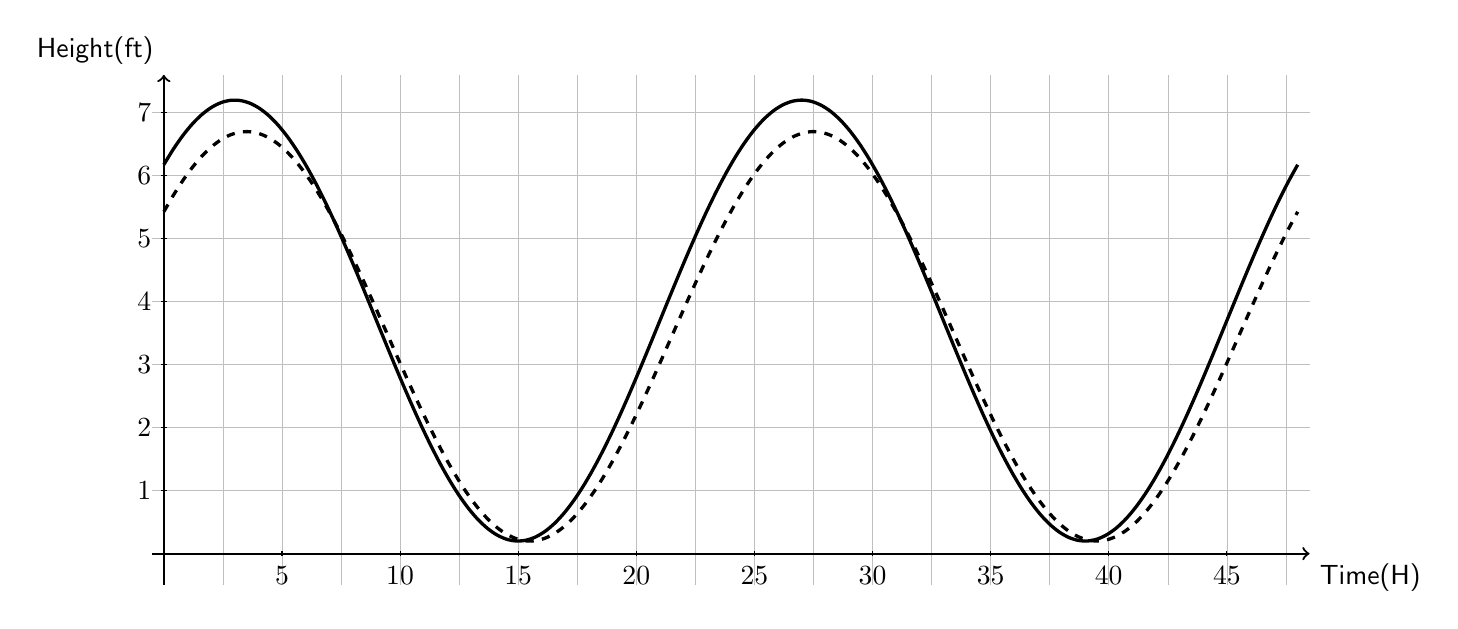
\begin{tikzpicture}[y=0.8cm, x=.3cm,font=\sffamily]
    % Define the x bounds
    \def\lowX{-0.5}
    \def\highX{48.5}
    % define the y bounds
    \def\lowY{-0.5}
    \def\highY{7.6}
    % Add a grid
    \draw[xstep = 2.5,ystep=1, gray, very thin,opacity=0.5] (\lowX, \lowY) grid ( \highX, \highY);
 	% Draw the axes
	\draw[thick,->] (\lowX,0) -- coordinate (x axis mid) (\highX,0) node[anchor = north west] {Time(H)};
    \draw[thick,->] (0,\lowY) -- coordinate (y axis mid) (0,\highY) node[anchor = south east] {Height(ft)};
    % Label the y axis
    \foreach \y in {1,2,...,7} {
      \draw (1pt, \y) -- (-1pt, \y) node[anchor = east] {$\y$};
    }
    % Label the x axis
    \foreach \x in {5,10,...,45} {
      \draw (\x,1pt) -- (\x,-1pt) node[anchor = north] {$\x$};
    }
    % Draw the function.
    \begin{scope}
      %\clip(-4,-1) rectangle (8,5);
      \draw[scale=1.0,domain=0:48,smooth,variable=\x,very thick,black,samples=120] 
            plot ({\x},{3.7+3.5*sin(deg(pi*\x/12+pi/4))});
      \draw[scale=1.0,domain=0:48,smooth,variable=\x,very thick,black,samples=120,dashed] 
            plot ({\x},{3.45+3.25*sin(deg(pi*(\x-0.5)/12+pi/4))});
    \end{scope}

    %\node[above=0.1cm] at (-2,2 )   {\nextXValue};

  \end{tikzpicture}


\end{problem}

\postClass

\begin{problem}
\item Briefly state two ideas from today's class.
  \begin{itemize}
  \item
  \item
  \end{itemize}
\item An enzyme in a solution decays, and the concentration (mg/liter)
  as a function of time in hours is
  \begin{eqnarray*}
    C(t) & = & \frac{3.5}{5.0+t}.
  \end{eqnarray*}
  \begin{subproblem}
  \item Make a sketch of the concentration as a function of
    time. Assume that the time is positive. Annotate your plot and
    label your axes.
    \item How long will it take for the enzyme to be reduced to half
      its original concentration?
    \item Another enzyme is present, and its concentration is linked
      to the first. Its concentration is half the first enzyme's
      concentration 30 minutes in the past. Determine the formula for
      the second enzyme's concentration. (This is referred to as a
      delay relationship.)
    \item How long will it take for the second enzyme to be reduced to
      half its original concentration?
    \item Make a sketch of the concentration of both enzymes as a
      function of time. Assume that the time is positive. Annotate
      your plot and label your axes.
  \end{subproblem}
\end{problem}


%%% Local Variables:
%%% mode: latex
%%% TeX-master: "../labManual"
%%% End:
